\documentclass[11pt,a4paper]{article}

\usepackage[margin=19.5mm]{geometry}
\usepackage{amsmath,amssymb,amsthm,mathtools}
\usepackage{booktabs,array,longtable}
\usepackage{enumitem}
\usepackage{xcolor}
\usepackage{fancyhdr}
\usepackage{tikz}
\usetikzlibrary{arrows.meta,calc,positioning}
\usepackage[hidelinks]{hyperref}

\hypersetup{
    colorlinks=true,
    linkcolor=blue!55!black,
    urlcolor=blue!55!black,
    citecolor=blue!55!black,
    pdftitle={2D Finite Volume Method Solver Suite: Technical Reference},
    pdfauthor={FVM Comparison Project}
}

\allowdisplaybreaks

\definecolor{accent}{RGB}{24,72,128}
\definecolor{subaccent}{RGB}{60,110,160}
\definecolor{muted}{RGB}{100,105,115}

\theoremstyle{definition}
\newtheorem{remark}{Remark}[section]

\pagestyle{fancy}
\fancyhf{}
\lhead{\small\textcolor{muted}{2D Finite Volume Solver Suite}}
\rhead{\small\textcolor{muted}{Technical Reference}}
\cfoot{\small\thepage}
\renewcommand{\headrulewidth}{0.4pt}
\setlength{\headheight}{14pt}
\emergencystretch=1.5em

\setlength{\intextsep}{9pt plus 2pt minus 2pt}
\setlist[itemize]{itemsep=1pt,topsep=2pt,parsep=0pt}
\setlist[enumerate]{itemsep=1pt,topsep=2pt,parsep=0pt}

\newcommand{\dd}{\mathrm{d}}
\newcommand{\R}{\mathbb{R}}
\newcommand{\norm}[1]{\left\lVert #1 \right\rVert}
\newcommand{\abs}[1]{\left\lvert #1 \right\rvert}
\newcommand{\code}[1]{\texttt{#1}}

\title{\vspace{-8mm}\textbf{\Large 2D Finite Volume Method (FVM) Solver Suite}\\[4pt]
\large Mathematical Formulations, High-Order Discretizations, Linear Solvers,\\ Mesh Generation, MPI Parallelization, and Benchmark Synthesis}
\author{}
\date{}

\begin{document}
\maketitle
\vspace{-10mm}

\noindent\fbox{\parbox{\dimexpr\textwidth-2\fboxsep-2\fboxrule}{%
\small
\textbf{Scope.} This document provides the complete mathematical and algorithmic specification of the C++20 2D finite-volume codebase covering: (i) repository and core data-structure architecture; (ii) quadrature rules and exact polygon/disk geometric initialization; (iii) structured and unstructured Delaunay mesh pipelines; (iv) dense and sparse linear-algebra solvers; (v) 1st-order monotone, 2nd-order TVD/MUSCL, 2nd/3rd-order ENO, and 5th-order structured / $P^2$ unstructured WENO spatial discretizations; (vi) explicit and SSP Runge--Kutta time integrators with exact stage-weighted discrete conservation; (vii) OpenMPI structured and unstructured domain decompositions; and (viii) quantitative results across the three scalar conservation-law benchmarks.
}}

\vspace{4mm}
\tableofcontents
\newpage

%======================================================================
\section{Repository Architecture and Core Infrastructure}
%======================================================================

The codebase is written in pure C++20 (\code{-std=c++20 -O2 -Wall -Wextra -Wpedantic -Werror}) with zero external PDE, meshing, or linear-algebra dependencies in serial builds, and optional OpenMPI parallelism toggled via \code{USE\_MPI=1} (\code{Makefile}) or \code{-DFVM\_USE\_MPI=ON} (\code{CMakeLists.txt}).

\subsection{Directory Layout}

\begin{center}
\footnotesize
\begin{tabular}{@{}l >{\raggedright\arraybackslash}p{0.56\textwidth}@{}}
\toprule
\textbf{Path} & \textbf{Responsibility} \\
\midrule
\code{include/fvm/core/types.hpp} & Scalar/index aliases (\code{Real=double}, \code{Index}, \code{SignedIndex}), \code{Vec2}, 2D cross/dot \\
\code{include/fvm/core/field.hpp} & Ghost-aware \code{StructuredField2D}, discrete $L^1/L^2/L^\infty$ error norms, \code{FieldStats} \\
\code{include/fvm/core/convergence.hpp} & Experimental order of convergence (EOC), tabular console \& CSV writers \\
\code{include/fvm/core/mpi\_context.hpp} & \code{MpiGuard}, \code{CartDecomp2D}, \code{UnstructuredDecomp}, halo exchanges, reductions \\
\code{include/fvm/linalg/dense.hpp} & \code{DenseMatrix}, partial-pivoting LU, rank-checked Householder \code{QRDecomposition} \\
\code{include/fvm/linalg/sparse.hpp} & \code{TripletBuilder}, \code{CSRMatrix}, Jacobi / SGS preconditioned CG \& BiCGSTAB \\
\code{include/fvm/mesh/geometry\_exact.hpp} & Sutherland--Hodgman polygon clipping, exact box/band/disk overlap \\
\code{include/fvm/mesh/structured\_mesh.hpp} & Uniform 2D Cartesian grid, ghost cells, 7 boundary condition types \\
\code{include/fvm/mesh/unstructured\_mesh.hpp} & Cell-face-vertex topology, geometric quality metrics, 1-to-4 refinement, BFS stencils \\
\code{include/fvm/mesh/mesh\_generator.hpp} & Bowyer--Watson Delaunay, Lloyd smoothing, structured tri meshes, Gmsh v2.2 reader \\
\code{include/fvm/numerics/quadrature.hpp} & 1D Gauss--Legendre ($n\in\{1,\dots,5\}$) and symmetric 2D triangle rules ($\deg\le 5$) \\
\code{include/fvm/numerics/flux.hpp} & Exact linear upwind flux, scalar Rusanov/LLF flux, 16-pt wave-speed bound \\
\code{include/fvm/numerics/time\_integrator.hpp} & Forward Euler, SSP-RK2, SSP-RK3, classical RK4, Butcher stage weights \\
\code{include/fvm/solvers/structured\_solver.hpp} & \code{StructuredFVSolver} (1st, TVD, ENO2/3, WENO5-Z/JS) \\
\code{include/fvm/solvers/unstructured\_solver.hpp} & \code{UnstructuredAdvectionSolver} (1st, TVD, ENO2/3, WENO-$P^2$) \\
\code{include/fvm/io/vtk\_writer.hpp} & ParaView XML \code{.vti} (\code{ImageData}), \code{.vtu} (\code{UnstructuredGrid}), and \code{.pvd} series \\
\code{src/*} & Out-of-line implementations corresponding to \code{include/fvm/*} \\
\code{apps/problem\{1,2,3\}*.cpp} & Standalone drivers for the three benchmark problems \\
\code{tests/test\_\{core,solvers\}.cpp} & Unit tests and convergence/conservation/MPI-equivalence verification suite \\
\bottomrule
\end{tabular}
\end{center}

\subsection{Discrete Norms, Field Storage, and VTK Output}

For a structured grid of interior size $n_x \times n_y$ with ghost margin $g = \code{nghost}$, \code{StructuredField2D} stores row-major cell averages with stride $s = n_x + 2g$:
\[
\text{storage\_index}(i,j) = (j + g)s + (i + g), \qquad -g \le i < n_x + g,\quad -g \le j < n_y + g.
\]
Given reference cell averages $u^{\mathrm{ref}}_K$, discrete $L^1$, $L^2$, and $L^\infty$ errors over interior cells $\mathcal{T}_h$ of areas $|K|$ are computed identically across structured and unstructured meshes as
\[
E_1 = \sum_{K\in\mathcal{T}_h} |K|\,\abs{\bar{u}_K - u_K^{\mathrm{ref}}}, \qquad
E_2 = \left(\sum_{K\in\mathcal{T}_h} |K|\,\abs{\bar{u}_K - u_K^{\mathrm{ref}}}^2\right)^{1/2}, \qquad
E_\infty = \max_{K\in\mathcal{T}_h} \abs{\bar{u}_K - u_K^{\mathrm{ref}}},
\]
and the experimental order of convergence between consecutive mesh sizes $h_c > h_f$ is $\mathrm{EOC} = \ln(E_c/E_f) / \ln(h_c/h_f)$. ParaView visualization writes \code{Float64} ASCII \code{CellData} into XML \code{.vti} (\code{ImageData}) and \code{.vtu} (\code{UnstructuredGrid} with VTK cell types \code{5}=\code{VTK\_TRIANGLE}, \code{9}=\code{VTK\_QUAD}, \code{7}=\code{VTK\_POLYGON}) indexed by a \code{.pvd} collection.

%======================================================================
\section{Quadrature and Exact Geometric Initialization}
%======================================================================

\subsection{Quadrature Rules (\code{quadrature.hpp})}

\begin{itemize}
\item \textbf{1D Gauss--Legendre on $[0,1]$ (\code{gauss\_legendre\_01}):} Exact for polynomials of degree $\le 2n-1$ for $n \in \{1,2,3,4,5\}$, mapped from $[-1,1]$ via $\xi = \frac{1}{2}(x + 1)$ and $w = \frac{1}{2}w_{[-1,1]}$. In particular: $n=2$ uses $\xi_\pm = \frac{1}{2} \pm \frac{1}{2\sqrt{3}}$, $w=\frac{1}{2}$ (exact deg~3); $n=3$ uses $\xi = \frac{1}{2} + \{-\frac{\sqrt{15}}{10}, 0, +\frac{\sqrt{15}}{10}\}$ with weights $\{\frac{5}{18}, \frac{8}{18}, \frac{5}{18}\}$ (exact deg~5).
\item \textbf{Symmetric Positive-Weight Triangle Rules (\code{triangle\_rule}):}
  \begin{itemize}
    \item $\deg \le 1$: 1-point centroid rule $(\frac{1}{3},\frac{1}{3},\frac{1}{3})$, $w=1$.
    \item $\deg \le 2$: 3-point cyclic permutations of $(\frac{2}{3},\frac{1}{6},\frac{1}{6})$, $w=\frac{1}{3}$.
    \item $\deg \le 5$: 7-point Radon / Hammer--Marlowe--Stroud interior rule ($w_0 = \frac{9}{40}$ at barycenter; orbits $a_{1,2} = (9\pm 2\sqrt{15})/21$, $b_{1,2} = (6\mp\sqrt{15})/21$, $w_{1,2} = (155\mp\sqrt{15})/1200$).
  \end{itemize}
\end{itemize}

\subsection{Exact Cell-Average Clipping (\code{geometry\_exact.hpp})}

Midpoint sampling of discontinuous initial data creates $O(h)$ cell-average perturbations along interfaces that pollute high-order scheme comparisons. The geometry engine computes exact volume fractions:
\begin{enumerate}
\item \textbf{Sutherland--Hodgman Half-Plane Clipping (\code{clip\_polygon\_halfplane}):} Clips a polygon $P$ sequentially against $ax + by + c \ge 0$ by linear edge interpolation $t = f(A)/(f(A)-f(B))$, followed by exact shoelace area $|P| = \frac{1}{2}\abs{\sum_k \mathbf{p}_k \times \mathbf{p}_{k+1}}$.
  \begin{itemize}
    \item \code{intersection\_area\_box}: clips $P$ against $x \ge x_{\min}$, $x \le x_{\max}$, $y \ge y_{\min}$, $y \le y_{\max}$ (used for unstructured patches and leakage diagnostics).
    \item \code{intersection\_area\_diagonal\_band}: clips $P$ against $y - x + w \ge 0$ and $x - y + w \ge 0$ (exact cell averages of $\mathbf{1}_{\{|y-x| < w\}}$).
  \end{itemize}
\item \textbf{1D Overlap (\code{interval\_overlap\_fraction}):} Evaluates $\max(0, \min(b,d)-\max(a,c))/(b-a)$ for exact piecewise-constant Dirichlet inflow face averages.
\item \textbf{Exact Disk--Rectangle Overlap (\code{disk\_intersection\_area\_rect}):} Splits $[x_0,x_1]\times[y_0,y_1]$ across $x=0$ and $y=0$ into up to 4 first-quadrant rectangles $[a,b]\times[c,d]$ ($a,c\ge 0$). Within each piece intersected with $x^2+y^2\le R^2$, with $x_{\max} = \min(b,\sqrt{\max(0,R^2-c^2)})$ and $x_d = \mathrm{clamp}(\mathbf{1}_{d<R}\sqrt{\max(0,R^2-d^2)},\, a,\, x_{\max})$:
\[
|{[a,b]\times[c,d]}\cap B_R(0)| = (x_d - a)(d - c) + \int_{x_d}^{x_{\max}} \left(\sqrt{R^2-x^2} - c\right)\dd x,
\]
evaluated in closed form via the exact antiderivative
\[
A(x) = \frac{1}{2}\Bigl(x\sqrt{R^2-x^2} + R^2\arcsin\bigl(\mathrm{clamp}(x/R,-1,1)\bigr)\Bigr).
\]
\end{enumerate}

%======================================================================
\section{Structured and Unstructured Mesh Pipelines}
%======================================================================

\subsection{Structured Cartesian Grid and Seven Boundary Conditions}

\code{StructuredMesh2D} partitions $[x_{\min},x_{\max}]\times[y_{\min},y_{\max}]$ into $n_x\times n_y$ uniform rectangles of size $\Delta x \times \Delta y$ surrounded by $g$ ghost layers ($g=1$ for 1st-order, $g=2$ for TVD/ENO2, $g=3$ for ENO3/WENO5). Boundary conditions are split into \code{apply\_boundary\_conditions\_x} (filling $i\in[-g,-1]\cup[n_x,n_x+g)$ over $0\le j<n_y$) and \code{apply\_boundary\_conditions\_y} (filling $j\in[-g,-1]\cup[n_y,n_y+g)$ over the extended range $-g \le i < n_x + g$, populating all corner ghosts). For left-boundary ghost index $i_l = -1 - k$ ($0\le k < g$) with cell center $\mathbf{x}_{i_l,j}$ and bounding box $[x_0,x_0+\Delta x]\times[y_0,y_0+\Delta y]$:
\begin{center}
\footnotesize
\begin{tabular}{@{}l p{0.73\textwidth}@{}}
\toprule
\textbf{BC Type} & \textbf{Ghost Cell Rule (illustrated at left boundary $i_l = -1-k$)} \\
\midrule
\code{Periodic} & $u_{i_l, j} = u_{(n_x - 1 - k \bmod n_x + n_x)\bmod n_x,\, j}$ \\
\code{ZeroGradient} & $u_{i_l, j} = u_{0, j}$ \\
\code{Extrapolate} & $u_{i_l, j} = 4 u_{i_l+1, j} - 6 u_{i_l+2, j} + 4 u_{i_l+3, j} - u_{i_l+4, j}$ (4th-order cubic, if $n_x\ge 4$) \\
\code{DirichletReflect} & $u_{i_l, j} = 2 u_b(x_{\min}, y_j, t) - u_{\min(k, n_x-1),\, j}$ \\
\code{DirichletExact} & $u_{i_l, j} = u_b(x_{i_l}, y_j, t)$ (midpoint evaluation at ghost cell center) \\
\code{DirichletCellAvg} & $4\times 4$ tensor-product Gauss--Legendre quadrature of $u_b(\cdot,\cdot,t)$ on ghost cell \\
\code{DirichletFaceAvg} & $u_{i_l, j} = \frac{1}{\Delta y}\int_{y_0}^{y_0+\Delta y} u_{\text{in}}(y, t)\,\dd y$ (\code{face\_avg(y0, y1, t)}) \\
\bottomrule
\end{tabular}
\end{center}
Analogous mirrored formulas hold for \code{right}, \code{bottom}, and \code{top}.

\subsection{Unstructured Mesh Topology, Quality Metrics, and Refinement}

\code{UnstructuredMesh2D} supports arbitrary triangles and convex/general polygons (built from vertex coordinates and cell vertex lists, enforcing counter-clockwise vertex ordering via signed shoelace area). For each cell $K$ with polygon vertices $\mathbf{p}_0,\dots,\mathbf{p}_{m-1}$, centroid $\mathbf{x}_K = \frac{1}{6|K|}\sum_{k=0}^{m-1} (\mathbf{p}_k + \mathbf{p}_{k+1})(\mathbf{p}_k\times\mathbf{p}_{k+1})$, and perimeter $P_K = \sum_e |e|$:
\[
h_K = \sqrt{|K|}, \qquad r_{\text{in}, K} = \frac{2|K|}{P_K}, \qquad
h_{\text{diam}} = \max_K \max_{a<b} \norm{\mathbf{p}_a - \mathbf{p}_b}_2, \qquad
q_K = \begin{cases}
\dfrac{4\sqrt{3}\,|K|}{\sum_{k=0}^2 |e_k|^2}, & m=3,\\[8pt]
\dfrac{4\pi |K|}{P_K^2}, & m \ge 4.
\end{cases}
\]
Interior faces $f$ link \code{left\_cell} $\to$ \code{right\_cell} with outward unit normal $\mathbf{n}_f = \mathbf{t}_f^{\perp,\text{cw}} / |f| = (t_y, -t_x)/|f|$; boundary faces carry \code{right\_cell = -1} and an integer \code{boundary\_tag}.

\begin{itemize}
\item \textbf{Self-Similar 1-to-4 Uniform Refinement (\code{refine\_uniform}):} Each edge inserts a shared midpoint vertex, subdividing each triangle $(v_0,v_1,v_2)$ into four congruent child triangles $(v_0, m_{01}, m_{20})$, $(m_{01}, v_1, m_{12})$, $(m_{20}, m_{12}, v_2)$, and $(m_{01}, m_{12}, m_{20})$, preserving $q_{\min}$ exactly across levels and inheriting parent boundary tags. (Quads split analogously around their centroid into 4 sub-quads.)
\item \textbf{Neighborhood BFS Stencil Collection (\code{collect\_stencil}):} Performs breadth-first search outward from cell $c$ up to \code{min\_neighbors}, strictly enqueueing direct face neighbors before vertex-sharing neighbors (\code{vertex\_to\_cells\_}) to ensure well-conditioned inner rings.
\end{itemize}

\subsection{Bowyer--Watson Delaunay Generator, Lloyd Smoothing, and Gmsh Loader}

\begin{enumerate}
\item \textbf{Point Distribution (\code{generate\_unstructured\_tri\_mesh}):} Places equispaced boundary nodes around $[x_{\min},x_{\max}]\times[y_{\min},y_{\max}]$ and interior nodes on a staggered lattice ($x_{\text{shift}} = 0.25\Delta x$ on odd $j$ rows) perturbed by seeded \code{std::mt19937} uniform noise $U(-0.5, 0.5)$ scaled by $\mathrm{clamp}(\text{jitter}, 0, 0.45)$ and clamped within $0.25\Delta x, 0.25\Delta y$ of the boundary.
\item \textbf{Bowyer--Watson Delaunay Triangulation:}
  \begin{itemize}
    \item Sorts points into $\lfloor \sqrt{N_{\text{pts}}}\rfloor$ $y$-rows in alternating serpentine $x$-order so sequential insertions stay geometrically adjacent.
    \item Initializes a large super-triangle $\bigl(\mathbf{c}+(-20S,-20S),\,\mathbf{c}+(20S,-20S),\,\mathbf{c}+(0,25S)\bigr)$ where $S = \max(L_x,L_y)$.
    \item For each point $\mathbf{p}$: walks from the previous triangle hint across edges violating \code{orient2d} ($\le \text{tol}$), verifies circumcircle containment via the $3\times 3$ lifted determinant $\code{in\_circumcircle} > 10^{-13}S^4$ (with linear fallback scan if needed), expands the bad-triangle Delaunay cavity via BFS, removes dead triangles, connects cavity boundary edges to $\mathbf{p}$, relinks adjacency pointers, discards triangles referencing super-triangle vertices or area $\le 10^{-12}L_xL_y/N_{\text{pts}}$, and enforces CCW orientation.
  \end{itemize}
\item \textbf{Area-Weighted Centroid (Lloyd) Smoothing:} Repeated \code{smoothing\_iters} times: while keeping boundary points fixed, each interior vertex moves to the area-weighted centroid average of its incident Delaunay triangles,
\[
\mathbf{p}_i^{\text{new}} = \frac{\sum_{T \ni i} |T|\,\mathbf{x}_T}{\sum_{T \ni i} |T|},
\]
followed by full Bowyer--Watson re-triangulation so the mesh remains strictly Delaunay with high isotropic regularity ($q_{\min} \approx 0.815$ for \code{jitter=0.35, smooth=5}).
\item \textbf{Gmsh v2.2 Reader \& Structured Triangulations:} \code{load\_gmsh\_v2} parses ASCII \code{\$Nodes} and \code{\$Elements} (2-node boundary lines preserving physical tags, 3-node triangles, 4-node quads); \code{generate\_structured\_tri\_mesh} constructs \code{UnionJack}, \code{ForwardSlash}, and \code{Alternating} diagonal triangulations.
\end{enumerate}

%======================================================================
\section{Dense and Sparse Linear Algebra}
%======================================================================

All reconstruction and solver linear algebra is implemented in \code{include/fvm/linalg/} and \code{src/linalg/}. Table~\ref{tab:linalg_usage} clarifies exactly where each solver component is active.

\begin{table}[h]
\centering\footnotesize
\caption{Linear solvers implemented in \code{fvm::linalg} and their role in the benchmark suite.}
\label{tab:linalg_usage}
\begin{tabular}{@{}l l >{\raggedright\arraybackslash}p{0.25\textwidth} >{\raggedright\arraybackslash}p{0.26\textwidth}@{}}
\toprule
\textbf{Method} & \textbf{Class / Function} & \textbf{Complexity / Precond} & \textbf{Usage in Codebase} \\
\midrule
Householder QR & \code{QRDecomposition} & Precompute $O(mn^2)$; solve $O(mn)$ & TVD gradients, ENO3/WENO $P^2$ fits \\
$2\times 2$ Cramer Inv. & Inline \code{ENO2Pair} & $O(1)$ exact inverse & Unstructured ENO2 sector slopes \\
Dense LU (part. piv.) & \code{solve\_lu} & $O(n^3/3)$, tol $10^{-14}\max(1,\norm{A}_\infty)$ & General small square systems (tests) \\
CSR Precond. CG & \code{solve\_cg} & CSR SpMV; None / Jacobi / SGS & SPD sparse systems (tests / library) \\
CSR Precond. BiCGSTAB & \code{solve\_bicgstab} & CSR SpMV; None / Jacobi / SGS & Nonsymmetric sparse systems (tests / library) \\
\bottomrule
\end{tabular}
\end{table}

\subsection{Partial-Pivoting LU and Rank-Checked Householder QR}

\begin{itemize}
\item \textbf{Partial-Pivoting Dense LU (\code{solve\_lu}):} Solves square $n\times n$ systems $A\mathbf{x}=\mathbf{b}$ in place by scanning column $k$ for maximal pivot $|A_{ik}|$, rejecting singular pivots $\le 10^{-14}\max(1, \max_{i,j}|A_{ij}|)$, row-swapping $A$ and $\mathbf{b}$, eliminating subdiagonal entries, and back-substituting.
\item \textbf{Precomputed Householder QR (\code{QRDecomposition}):} Used heavily on every unstructured cell stencil for both TVD linear gradients ($n=2$) and ENO3/WENO $P^2$ polynomials ($n=5$). For an overdetermined $m \times n$ matrix $A$ ($m \ge n$):
  \begin{enumerate}
    \item \code{try\_compute} scans column $k$'s lower subvector $\mathbf{x} = A_{k:m, k}$ and rejects rank deficiency if $\norm{\mathbf{x}}_2 \le 10^{-13}\max(1, \norm{A}_\infty)$.
    \item Sets $\alpha = -\operatorname{sign}(x_0)\norm{\mathbf{x}}_2$ (using $\alpha = -\norm{\mathbf{x}}_2$ for $x_0\ge 0$ to avoid cancellation), normalizes Householder vector $\mathbf{v}$ with $v_0 = 1$, $v_i = A_{ik}/(x_0 - \alpha)$ ($i>k$), $\beta_k = 2/(1 + \sum_{i>k} v_i^2)$, stores $\alpha$ in \code{r\_diag\_[k]}, and applies $I - \beta_k \mathbf{v}\mathbf{v}^T$ to trailing columns $j>k$.
    \item Exposes \code{min\_abs\_r\_diag()} and \code{max\_abs\_r\_diag()} so stencil builders enforce explicit geometric conditioning bounds $\min_k |R_{kk}| > 10^{-3}$ and $\max_k|R_{kk}|/\min_k|R_{kk}| < \kappa_{\max}$ ($\kappa_{\max}=500$ for central $P^2$ stencils, $150$ for directional sector stencils).
    \item At every Runge--Kutta stage, \code{QRDecomposition::solve(rhs)} computes $\mathbf{c} = Q^T\mathbf{b}$ in place via stored $(\mathbf{v}_k, \beta_k)$ and back-substitutes $R\mathbf{x} = \mathbf{c}_{0:n}$ in $O(mn)$ operations—completely avoiding normal-equations squaring of $\kappa(A)$ and avoiding $O(mn^2)$ matrix factorizations inside the time loop.
  \end{enumerate}
\end{itemize}

\subsection{Sparse CSR Storage, Symmetric Gauss--Seidel, CG, and BiCGSTAB}

Because time stepping across Problems 1--3 uses explicit SSP Runge--Kutta, \code{sparse.hpp/.cpp} provides verified sparse linear-algebra infrastructure (tested in \code{test\_core} on a 2D 5-point Poisson matrix where SGS-CG converges in 30 iterations and SGS-BiCGSTAB in 8 iterations) for implicit/diffusion extensions:
\begin{itemize}
\item \textbf{Canonical CSR Construction (\code{TripletBuilder::to\_csr}):} Sorts $(r,c,v)$ triplets lexicographically, coalesces duplicates, builds \code{row\_ptr\_}, \code{col\_idx\_}, \code{values\_}, and caches \code{diag\_\allowbreak offset\_[r]} for $O(1)$ diagonal lookup.
\item \textbf{Preconditioners (\code{apply\_preconditioner}):} Supports \code{None}, \code{Jacobi} ($z_i = r_i / D_{ii}$ for $|D_{ii}| > 10^{-30}$), and \textbf{Symmetric Gauss--Seidel (SGS)}, factoring $A = L + D + U$ and solving $M\mathbf{z} = \mathbf{r}$ with
\[
M = (D + L)\,D^{-1}\,(D + U)
\]
via a forward sweep $(D+L)\mathbf{y} = \mathbf{r}$ (exploiting sorted columns to stop when $j\ge i$), diagonal scaling $\mathbf{y} \leftarrow D\mathbf{y}$, and backward sweep $(D+U)\mathbf{z} = \mathbf{y}$.
\item \textbf{Krylov Iterations:} Both Preconditioned Conjugate Gradient (\code{solve\_cg}) for SPD matrices and Preconditioned BiCGSTAB (\code{solve\_bicgstab}, with shadow residual $\hat{\mathbf{r}}_0 = \mathbf{r}_0$ and early $\norm{\mathbf{s}}_2 \le \text{tol}$ termination) stop when $\norm{\mathbf{r}_k}_2 \le \max(\code{atol}, \code{rtol}\norm{\mathbf{r}_0}_2)$ (defaults: $\code{rtol}=10^{-10}$, $\code{atol}=10^{-14}$, $\code{max\_iter}=5000$), guarding denominators against $|\cdot|\le 10^{-30}$.
\end{itemize}

%======================================================================
\section{Governing Equations and Spatial Discretizations}
%======================================================================

We consider 2D scalar conservation laws on $\Omega \subset \R^2$:
\begin{equation}
\label{eq:claw}
\frac{\partial u}{\partial t} + \nabla\cdot \mathbf{f}(\mathbf{x}, u) = 0,
\qquad \mathbf{f}(\mathbf{x},u) = \bigl(f^x(\mathbf{x},u),\, f^y(\mathbf{x},u)\bigr).
\end{equation}
Integrating over control volume $K$ and applying the divergence theorem yields the exact semidiscrete finite-volume ODE for the cell average $\bar{u}_K(t) = \frac{1}{|K|}\int_K u(\mathbf{x},t)\,\dd\mathbf{x}$:
\begin{equation}
\label{eq:fvm_ode}
\frac{\dd \bar{u}_K}{\dd t} = -\frac{1}{|K|} \sum_{e \subset \partial K} |e| \sum_{q=1}^{N_q} w_q\, \hat{F}\!\left(u_K^-(\mathbf{x}_{e,q}),\, u_K^+(\mathbf{x}_{e,q});\, \mathbf{n}_{K,e}\right),
\end{equation}
where $\mathbf{x}_{e,q}$ and $w_q$ are 1D Gauss--Legendre quadrature nodes and normalized weights on edge $e$ ($\sum_q w_q = 1$), $u_K^\pm$ are inner/outer polynomial reconstructions, and $\hat{F}$ is a consistent, conservative numerical flux:
\begin{itemize}
\item \textbf{Exact Linear Upwind (\code{flux::linear\_upwind}):} For $\mathbf{f}(\mathbf{x},u) = \mathbf{v}(\mathbf{x}) u$ with $v_n = \mathbf{v}\cdot\mathbf{n}$,
  $\hat{F}(u_L,u_R;v_n) = v_n u_L$ if $v_n \ge 0$, else $v_n u_R$.
\item \textbf{Scalar Rusanov / Local Lax--Friedrichs (\code{flux::rusanov}):}
  \[
  \hat{F}(u_L, u_R) = \frac{1}{2}\bigl(f(u_L) + f(u_R)\bigr) - \frac{1}{2}\alpha\,(u_R - u_L),
  \qquad \alpha \ge \max_{u \in [\min(u_L,u_R),\,\max(u_L,u_R)]} \abs{f'(u)}.
  \]
  For nonconvex fluxes (Problem~3 KPP), endpoints alone underestimate $\alpha$ when $f'$ has interior extrema; \code{flux::interval\_max\_wave\_speed} samples 16 intermediate points, and global $\alpha = 1$ bounds $|\cos u|, |\sin u| \le 1$.
\end{itemize}

%----------------------------------------------------------------------
\subsection{Structured Cartesian Schemes (\code{StructuredFVSolver})}
%----------------------------------------------------------------------

On uniform grids, the explicit CFL time step is computed globally across ranks as
\[
\Delta t = \frac{\mathrm{CFL}}{\max_{\Omega} |a_x|/\Delta x + \max_{\Omega} |a_y|/\Delta y}.
\]

\paragraph{1st-Order Monotone ($\code{nghost}=1$, Forward Euler).}
Piecewise-constant reconstruction $u_L = \bar{u}_{i-1,j}$, $u_R = \bar{u}_{i,j}$ evaluated at the 1-point face midpoint. Formally 1st-order accurate, monotone, and strictly TVD.

\paragraph{2nd-Order MUSCL / TVD ($\code{nghost}=2$, \code{SSP\_RK2}).}
Along each sweep direction (shown for $x$ with $\Delta_- = \bar{u}_i - \bar{u}_{i-1}$, $\Delta_+ = \bar{u}_{i+1} - \bar{u}_i$), cell $i$ reconstructs a limited linear profile giving interface traces $u_{i+1/2}^L = \bar{u}_i + \frac{1}{2}\sigma_i$ and $u_{i-1/2}^R = \bar{u}_i - \frac{1}{2}\sigma_i$, where $\sigma_i = 0$ if $\Delta_-\Delta_+ \le 0$ and otherwise:
\[
\sigma_i =
\begin{cases}
\operatorname{minmod}_2(\Delta_-, \Delta_+), & \text{\code{Minmod} (Problem 3)},\\[3pt]
\dfrac{2\Delta_-\Delta_+}{\Delta_- + \Delta_+}, & \text{\code{VanLeer}},\\[6pt]
\operatorname{minmod}_3\!\bigl(\tfrac{1}{2}(\Delta_-+\Delta_+),\, 2\Delta_-,\, 2\Delta_+\bigr), & \text{\code{MC} (Problem 1)},\\[3pt]
\operatorname{sign}(\Delta_-)\max\bigl(\min(2|\Delta_-|,|\Delta_+|),\,\min(|\Delta_-|,2|\Delta_+|)\bigr), & \text{\code{Superbee}}.
\end{cases}
\]
Midpoint face quadrature gives true 2nd-order smooth 2D FV accuracy because midpoint integration is exact for linear face fluxes.

\paragraph{3rd-Order ENO (\code{ENO3}, $\code{nghost}=3$, \code{SSP\_RK3}).}
True 3rd-order 2D finite-volume accuracy requires two directional passes across each face (Shu~1997, Algorithm~2.1):
\begin{enumerate}
\item \textbf{Pass 1 --- Normal Face Averages (\code{eno3\_cell\_faces}):} On stencil $\{\bar{u}_{-2}, \bar{u}_{-1}, \bar{u}_0, \bar{u}_1, \bar{u}_2\}$, two Newton divided-difference comparisons select shift $r\in\{0,1,2\}$: if $|\bar{u}_0-\bar{u}_{-1}| \ge |\bar{u}_1-\bar{u}_0|$, choose $r=1$ when $|\bar{u}_1 - 2\bar{u}_0 + \bar{u}_{-1}| < |\bar{u}_2 - 2\bar{u}_1 + \bar{u}_0|$, else $r=0$; otherwise choose $r=2$ when $|\bar{u}_0 - 2\bar{u}_{-1} + \bar{u}_{-2}| < |\bar{u}_1 - 2\bar{u}_0 + \bar{u}_{-1}|$, else $r=1$. The quadratic reconstruction gives face averages:
\begin{align*}
r=0:\quad & u_L = \tfrac{1}{6}(11\bar{u}_0 - 7\bar{u}_1 + 2\bar{u}_2), && u_R = \tfrac{1}{6}(2\bar{u}_0 + 5\bar{u}_1 - \bar{u}_2),\\
r=1:\quad & u_L = \tfrac{1}{6}(2\bar{u}_{-1} + 5\bar{u}_0 - \bar{u}_1), && u_R = \tfrac{1}{6}(-\bar{u}_{-1} + 5\bar{u}_0 + 2\bar{u}_1),\\
r=2:\quad & u_L = \tfrac{1}{6}(-\bar{u}_{-2} + 5\bar{u}_{-1} + 2\bar{u}_0), && u_R = \tfrac{1}{6}(2\bar{u}_{-2} - 7\bar{u}_{-1} + 11\bar{u}_0).
\end{align*}
Notice this normal pass is executed across the padded transverse band $j \in [-2, n_y + 1]$ so 5 tangential face averages are available for every interior face.
\item \textbf{Tangential 2-Point Gauss Deconvolution (\code{eno3\_gauss2}):} Evaluating a 1D-reconstructed face average only at the face midpoint introduces an $O(h^2)$ tangential midpoint error, capping 2D FV schemes at 2nd order. Applying ENO3 to the 5 tangential face averages at $\xi_\pm = \pm \frac{1}{2\sqrt{3}}$, the quadratic deconvolution terms cancel on even powers because $\xi_\pm^2 - \frac{1}{12} = 0$, leaving simply
\[
p(\xi_\pm) = \bar{u}_0 \pm \frac{c_1}{2\sqrt{3}}, \qquad
c_1 = \begin{cases}
\tfrac{1}{2}(-3\bar{u}_0 + 4\bar{u}_1 - \bar{u}_2), & r=0,\\
\tfrac{1}{2}(\bar{u}_1 - \bar{u}_{-1}), & r=1,\\
\tfrac{1}{2}(3\bar{u}_0 - 4\bar{u}_{-1} + \bar{u}_{-2}), & r=2,
\end{cases}
\]
integrated with equal weights $\frac{1}{2}\bigl(\hat{F}(\xi_-) + \hat{F}(\xi_+)\bigr)$. (\code{ENO2} uses 1-point quadrature with $\sigma_i = \operatorname{minmod}_{\mathrm{abs}}(\Delta_-,\Delta_+)$ selecting the smaller slope magnitude.)
\end{enumerate}

\paragraph{5th-Order WENO5-Z and WENO5-JS (\code{WENO5}, $\code{nghost}=3$, \code{SSP\_RK3}).}
Implements genuine 5th-order 2D finite-volume WENO (Jiang--Shu~1996, Borges et~al.~2008, Buchm\"uller--Helzel~2014):
\begin{enumerate}
\item \textbf{Smoothness Indicators \& Nonlinear Weights:} On $\{q_{-2}, q_{-1}, q_0, q_1, q_2\}$,
\begin{align*}
\beta_0 &= \tfrac{13}{12}(q_{-2} - 2q_{-1} + q_0)^2 + \tfrac{1}{4}(q_{-2} - 4q_{-1} + 3q_0)^2,\\
\beta_1 &= \tfrac{13}{12}(q_{-1} - 2q_0 + q_1)^2 + \tfrac{1}{4}(q_{-1} - q_1)^2,\\
\beta_2 &= \tfrac{13}{12}(q_0 - 2q_1 + q_2)^2 + \tfrac{1}{4}(3q_0 - 4q_1 + q_2)^2.
\end{align*}
Unnormalized nonlinear factors $s_k$ are
\[
s_k = \begin{cases}
1 + \left(\dfrac{\tau_5}{\beta_k + \varepsilon}\right)^2, & \tau_5 = |\beta_0 - \beta_2|,\ \varepsilon = \max(10^{-36}, h^4)\quad (\text{\code{WENO\_Z}}),\\[8pt]
\dfrac{1}{(\beta_k + 10^{-6})^2}, & (\text{\code{WENO\_JS}}).
\end{cases}
\]
\item \textbf{Pass 1 — Normal Interface Averages (\code{weno5\_cell\_faces}):} Convexly weights the three 3-cell polynomials $p_k^{R/L}$ using optimal weights $(0.1, 0.6, 0.3)$ (mirrored $(0.3, 0.6, 0.1)$ for the left cell interface): $\omega_k = \gamma_k s_k / \sum_m \gamma_m s_m$.
\item \textbf{Pass 2 — Tangential 3-Point Gauss Deconvolution (\code{weno5\_gauss3}):} Integrates fluxes at $\xi \in \{-\frac{\sqrt{15}}{10}, 0, +\frac{\sqrt{15}}{10}\}$ with weights $(\frac{5}{18}, \frac{8}{18}, \frac{5}{18})$ along each face. The sub-stencil quadratic polynomials evaluated from cell averages $\bar{q}_0 + d_1^{(k)}\xi + d_2^{(k)}(\xi^2 - \frac{1}{12})$ have exact linear 5th-order deconvolution weights:
  \begin{itemize}
    \item \emph{Outer Gauss nodes} ($\xi = -\frac{\sqrt{15}}{10}$, mirrored at $+\frac{\sqrt{15}}{10}$): strictly positive optimal weights
    \[
    d_0^- = \frac{126}{655} + \frac{71\sqrt{15}}{5240}, \qquad
    d_1^- = \frac{403}{655}, \qquad
    d_2^- = \frac{126}{655} - \frac{71\sqrt{15}}{5240}.
    \]
    \item \emph{Face midpoint} ($\xi = 0$): exact optimal weights $\gamma = (-\frac{9}{80}, \frac{49}{40}, -\frac{9}{80})$ contain negative outer weights and are stabilized by \textbf{Shi--Hu--Shu (2002)} positive/negative splitting ($\theta = 3$, $\tilde{\gamma}^+ = (\frac{9}{80}, \frac{196}{80}, \frac{9}{80})$ with $\sigma^+ = \frac{214}{80}$, $\gamma^+ = (\frac{9}{214}, \frac{196}{214}, \frac{9}{214})$; $\tilde{\gamma}^- = (\frac{18}{80}, \frac{98}{80}, \frac{18}{80})$ with $\sigma^- = \frac{134}{80}$, $\gamma^- = (\frac{9}{67}, \frac{49}{67}, \frac{9}{67})$):
    \[
    u(\xi=0) = \sigma^+ v^+ - \sigma^- v^-.
    \]
  \end{itemize}
\end{enumerate}

%----------------------------------------------------------------------
\subsection{Unstructured Triangular Schemes (\code{UnstructuredAdvectionSolver})}
%----------------------------------------------------------------------

For linear advection $\partial_t u + \nabla\cdot(\mathbf{v}(\mathbf{x})u) = 0$, every face $f$ precomputes 3-point Gauss--Legendre quadrature data (\code{edge\_quad\_pts=3}, exact deg~5) $w_q |f|\,\mathbf{v}(\mathbf{x}_{f,q})\cdot\mathbf{n}_f$ with total normal flux rate $Q_f = \sum_q w_q |f|\mathbf{v}(\mathbf{x}_{f,q})\cdot\mathbf{n}_f$. The explicit time-step bound uses total cell outflow capacity:
\[
\Delta t_{\text{CFL}} = \min_{c} \frac{|K_c|}{\sum_{f\subset\partial K_c} \max(0, Q_{c,f})}, \qquad \Delta t = \mathrm{CFL}\cdot \Delta t_{\text{CFL}}.
\]
On boundary faces with $Q_{f,q} < 0$, the upwind value is supplied directly by \code{inflow\_bc\_(xq, yq, t, face.boundary\_tag)}.

\paragraph{1st-Order Upwind (Forward Euler).} Constant cell average $\bar{u}_c$ with upwind choice based on $Q_f \ge 0$.

\paragraph{2nd-Order Least-Squares TVD (\code{SSP\_RK2}).}
For cell $c$ with neighbor stencil $\mathcal{N}_c$ returned by \code{collect\_stencil(c, 6, true)}, precomputed \code{QRDecomposition} solves the distance-weighted overdetermined system ($w_r = 1/\max(\norm{\mathbf{x}_r-\mathbf{x}_c}_2, 10^{-14})$):
\[
w_r\,(\mathbf{x}_r - \mathbf{x}_c)\cdot \nabla u_c \approx w_r\,(\bar{u}_r - \bar{u}_c), \qquad r \in \mathcal{N}_c.
\]
Let $u_{\min} = \min_{r\in\mathcal{N}_c\cup\{c\}} \bar{u}_r$, $u_{\max} = \max_{r\in\mathcal{N}_c\cup\{c\}} \bar{u}_r$, $\Delta_{\max} = u_{\max}-\bar{u}_c \ge 0$, $\Delta_{\min} = u_{\min}-\bar{u}_c \le 0$. At each cell vertex $\mathbf{v}_k$ with unconstrained jump $\Delta u_k = \nabla u_c \cdot (\mathbf{v}_k - \mathbf{x}_c)$, define $a = |\Delta_+| \equiv |(\Delta u_k > 0 ? \Delta_{\max} : \Delta_{\min})|$ and $b = |\Delta u_k|$. The cell limiter $\phi_c = \min_k \phi_k$ takes:
\[
\phi_k =
\begin{cases}
\min\!\left(1,\, \dfrac{a}{b}\right), & \text{\code{BarthJespersen} (Problem 2)},\\[8pt]
\min\!\left(1,\, \dfrac{a^2 + 2ab + \varepsilon^2}{a^2 + 2b^2 + ab + \varepsilon^2}\right), & \text{\code{Venkatakrishnan}},
\end{cases}
\]
with threshold $\varepsilon^2 = u_{\text{scale}}^2 (2 h_c)^3$ and $u_{\text{scale}} = \max(1,\, u_{\max}-u_{\min})$.
Reconstructed polynomial $u_c(\mathbf{x}) = \bar{u}_c + \phi_c\nabla u_c \cdot (\mathbf{x}-\mathbf{x}_c)$ is integrated across interior and inflow faces using 3-point Gauss edge quadrature.

\paragraph{Unstructured $P^2$ ENO3 and $P^2$ WENO (\code{SSP\_RK3}).}
Each cell $c$ reconstructs a zero-mean quadratic polynomial in centered coordinates $\Delta\mathbf{x} = \mathbf{x} - \mathbf{x}_c$, scaled by $h_c = \sqrt{|K_c|}$ ($\hat{\Delta x} = \Delta x / h_c$, $\hat{\Delta y} = \Delta y / h_c$):
\begin{equation}
\label{eq:p2_poly}
p_c(\mathbf{x}) = \bar{u}_c + a_0 \hat{\Delta x} + a_1 \hat{\Delta y}
+ a_2(\hat{\Delta x}^2 - \hat{M}_{20,c})
+ a_3(\hat{\Delta x}\hat{\Delta y} - \hat{M}_{11,c})
+ a_4(\hat{\Delta y}^2 - \hat{M}_{02,c}),
\end{equation}
where the exact scaled moments $\hat{M}_{pq,c} = \frac{1}{|K_c| h_c^{p+q}}\int_{K_c} \Delta x^p \Delta y^q\,\dd\mathbf{x}$ are integrated with the 7-point degree-5 triangle rule. Conservation of $\bar{u}_c$ is exact ($\frac{1}{|K_c|}\int_{K_c} p_c = \bar{u}_c$), and integrating $p_c$ over neighbor cell $K_j$ gives the 5-unknown weighted least-squares equation ($w_r = 1/\max(1, \|\mathbf{x}_j-\mathbf{x}_c\|/h_c)$):
\begin{multline*}
w_r\Bigl[a_0\hat{d}_x + a_1\hat{d}_y + a_2(\hat{M}_{20,j}-\hat{M}_{20,c}+\hat{d}_x^2) + a_3(\hat{M}_{11,j}-\hat{M}_{11,c}+\hat{d}_x\hat{d}_y) \\
+ a_4(\hat{M}_{02,j}-\hat{M}_{02,c}+\hat{d}_y^2)\Bigr] \approx w_r(\bar{u}_j-\bar{u}_c).
\end{multline*}
For each cell $c$, the solver precomputes Householder QR factorizations over a cloud of $\ge 18$ BFS neighbors for:
\begin{itemize}
\item \textbf{One central stencil} (\code{preferred}, trying $9, 12, 16, \dots$ nearest neighbors until $\min|R_{kk}|>10^{-3}$ and $\kappa_R < 500$);
\item \textbf{Up to 6 overlapping directional $60^\circ$ sector stencils} ($\mathbf{d}_\theta = (\cos(s\pi/3),\sin(s\pi/3))$, keeping candidates with $\cos\alpha \ge -0.2$ ranked by $r(1.6-\cos\alpha)$, taking $6\text{--}8$ cells with $\kappa_R < 150$).
\end{itemize}
Using the dimensionless $H^1+H^2$ smoothness indicator on $K_c$,
\begin{align*}
\beta(p) &= \frac{1}{|K_c|}\int_{K_c} \abs{\hat{\nabla} p}^2\,\dd\mathbf{x} + \abs{\hat{\nabla}^2 p}_F^2 \\
&= \max\!\bigl(0,\, a_0^2+a_1^2 + (4a_2^2+a_3^2)\hat{M}_{20,c} + 4a_3(a_2+a_4)\hat{M}_{11,c} + (a_3^2+4a_4^2)\hat{M}_{02,c}\bigr)
+ 4a_2^2 + 2a_3^2 + 4a_4^2:
\end{align*}
\begin{itemize}
\item \textbf{\code{ENO3-Tri}:} Biased switching selects the smoothest sector polynomial if $4\min_s\beta_{\text{sec},s} < \beta_{\text{pref}}$, otherwise retains the central polynomial (the factor 4 avoids chattering in smooth regions).
\item \textbf{\code{WENO-Tri} (Dumbser--K\"aser / WENO-Z $P^2$):} Forms a smooth convex combination $a = \sum_m \omega_m a^{(m)}$ over central ($\lambda_0 = 100$) and sector ($\lambda_s = 1$) polynomials with exponent 4:
\[
\tilde{\omega}_m =
\begin{cases}
\lambda_m \left(1 + \left(\dfrac{\tau}{\beta_m + \varepsilon}\right)^4\right), & \tau = \max_s|\beta_0 - \beta_s|,\ \varepsilon = \max(10^{-30}, h_c^4)\quad (\text{\code{WENO\_Z}}),\\[8pt]
\dfrac{\lambda_m}{(\beta_m + 10^{-8})^4}, & (\text{\code{WENO\_JS}}).
\end{cases}
\]
(\code{ENO2} pairs $P^1$ fits over up to 10 well-angled neighbor pairs $|\det|/(\ell_a\ell_b)\ge 0.35$ with the same $4\times$ gradient-norm preference.)
\end{itemize}

\begin{figure}[h]
\centering
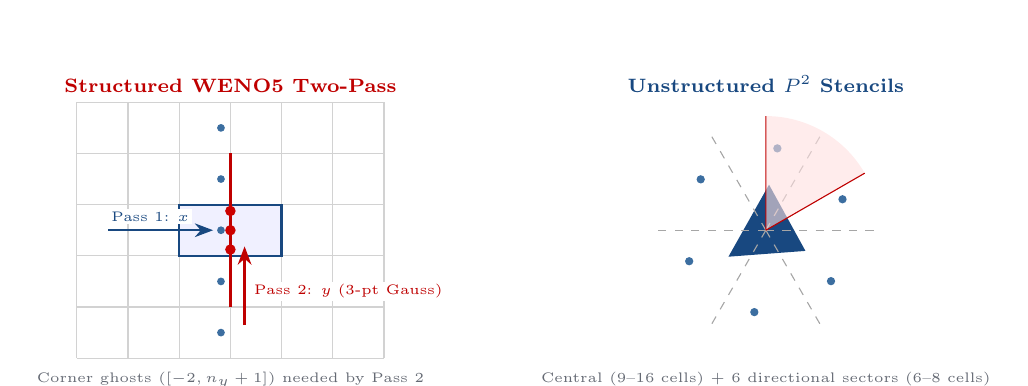
\begin{tikzpicture}[scale=1.0, >=Stealth]
% Left panel: Structured WENO5 2-pass Gauss stencil
\begin{scope}[shift={(0,0)}]
\draw[step=0.65cm, gray!35, thin] (-1.95,-1.3) grid (1.95,1.95);
\draw[thick, accent, fill=blue!6] (-0.65,0) rectangle (0.65,0.65);
\draw[very thick, red!75!black] (0,-0.65) -- (0,1.3);
\node[above, font=\scriptsize\bfseries, red!75!black] at (0,1.95) {Structured WENO5 Two-Pass};
% Pass 1 X-stencils along 5 rows
\foreach \j in {-2,-1,0,1,2} {
  \fill[subaccent] (-0.12, 0.325 + 0.65*\j) circle (1.4pt);
}
\draw[->, accent, thick] (-1.55,0.325) -- (-0.22,0.325);
\node[above, font=\tiny, accent, fill=white, inner sep=1pt] at (-1.02,0.40) {Pass 1: $x$};
\draw[->, red!75!black, thick] (0.18,-0.88) -- (0.18,0.12);
\node[right, font=\tiny, red!75!black, fill=white, inner sep=1pt] at (0.26,-0.45) {Pass 2: $y$ (3-pt Gauss)};
% Highlight 3 Gauss points on face i-1/2
\fill[red!80!black] (0,0.08) circle (1.9pt);
\fill[red!80!black] (0,0.325) circle (1.9pt);
\fill[red!80!black] (0,0.57) circle (1.9pt);
\node[below, font=\tiny, muted] at (0,-1.35) {Corner ghosts $([-2,n_y+1])$ needed by Pass 2};
\end{scope}

% Right panel: Unstructured P2 sectors
\begin{scope}[shift={(6.8,0.325)}]
\coordinate (C) at (0,0);
\draw[fill=blue!8, thick, accent] (-0.45,-0.32) -- (0.48,-0.25) -- (0.04,0.55) -- cycle;
\fill[accent] (C) circle (1.7pt) node[below right, font=\tiny] {$c$};
\foreach \ang in {0,60,120,180,240,300} {
  \draw[dashed, gray!70] (0,0) -- ({\ang}:1.45);
  \fill[subaccent] ({\ang+22}:1.05) circle (1.5pt);
}
% Highlight one 60 deg directional sector
\fill[red!12, opacity=0.6] (0,0) -- (30:1.45) arc (30:90:1.45) -- cycle;
\draw[red!75!black, thin] (0,0) -- (30:1.45) (0,0) -- (90:1.45);
\node[above, font=\scriptsize\bfseries, accent] at (0,1.62) {Unstructured $P^2$ Stencils};
\node[below, font=\tiny, muted] at (0,-1.68) {Central (9--16 cells) + 6 directional sectors (6--8 cells)};
\end{scope}
\end{tikzpicture}
\caption{Left: Two-pass 2D FV WENO5 reconstruction on a structured grid requiring diagonal ghost corners. Right: Central and $60^\circ$ directional sector $P^2$ QR stencils on unstructured triangles.}
\end{figure}

%======================================================================
\section{Time Integration and Exact Discrete Conservation}
%======================================================================

\subsection{Strong Stability Preserving Runge--Kutta Pairing}

For the semidiscrete ODE $\dd\mathbf{u}/\dd t = L(\mathbf{u},t)$, \code{RKStepper} (\code{time\_integrator.hpp}) implements four explicit integrators and associates effective Butcher stage weights $b_s$ (\code{rk\_stage\_weights}):
\begin{itemize}
\item \textbf{Forward Euler (\code{Euler}, 1st-order, $b=\{1\}$):} $\mathbf{u}^{n+1} = \mathbf{u}^n + \Delta t L(\mathbf{u}^n, t^n)$. Paired with \code{1st-Order}.
\item \textbf{SSP-RK2 / Heun (\code{SSP\_RK2}, 2nd-order, $b=\{\tfrac{1}{2},\tfrac{1}{2}\}$):} Paired with \code{TVD} and \code{ENO2}:
  \[
  \mathbf{u}^{(1)} = \mathbf{u}^n + \Delta t L(\mathbf{u}^n, t^n), \qquad
  \mathbf{u}^{n+1} = \frac{1}{2}\mathbf{u}^n + \frac{1}{2}\bigl(\mathbf{u}^{(1)} + \Delta t L(\mathbf{u}^{(1)}, t^n + \Delta t)\bigr).
  \]
\item \textbf{SSP-RK3 / Shu--Osher (\code{SSP\_RK3}, 3rd-order, $b=\{\tfrac{1}{6},\tfrac{1}{6},\tfrac{2}{3}\}$):} Paired with \code{ENO3} and \code{WENO}:
  \begin{align*}
  \mathbf{u}^{(1)} &= \mathbf{u}^n + \Delta t L(\mathbf{u}^n, t^n),\\
  \mathbf{u}^{(2)} &= \frac{3}{4}\mathbf{u}^n + \frac{1}{4}\bigl(\mathbf{u}^{(1)} + \Delta t L(\mathbf{u}^{(1)}, t^n + \Delta t)\bigr),\\
  \mathbf{u}^{n+1} &= \frac{1}{3}\mathbf{u}^n + \frac{2}{3}\bigl(\mathbf{u}^{(2)} + \Delta t L(\mathbf{u}^{(2)}, t^n + \tfrac{1}{2}\Delta t)\bigr).
  \end{align*}
\item \textbf{Classical RK4 (\code{RK4}, 4th-order, $b=\{\tfrac{1}{6},\tfrac{1}{3},\tfrac{1}{3},\tfrac{1}{6}\}$):} Available in the library and used for unsteady smooth 2D nonlinear WENO5 EOC tests (\code{test\_solvers.cpp}) where 3rd-order time stepping at fixed CFL would bottleneck spatial $O(h^5)$ accuracy.
\end{itemize}

\begin{remark}[Why Different Time Schemes Are Paired with Each Spatial Solver]
\leavevmode
\begin{enumerate}
\item \emph{Error balance:} At fixed CFL ($\Delta t \propto h$), total error scales as $O(h^{p_{\text{space}}} + h^{p_{\text{time}}})$, motivating Euler ($p=1$), SSP-RK2 ($p=2$), and SSP-RK3 ($p=3$). For steady waves $g(y-x)$ with $\mathbf{a}=(1,1)$, $\partial_t u \equiv 0$ eliminates temporal error so WENO5 reaches 5th-order EOC under SSP-RK3; unsteady smooth flows switch to RK4.
\item \emph{Imaginary-axis linear stability:} Low-dissipation ENO3 and WENO5 operators place eigenvalues near the imaginary axis $i\R$. Forward Euler ($|1+iy|>1$) and SSP-RK2 ($|1+iy-\frac{1}{2}y^2|>1$) contain no non-zero imaginary interval, whereas SSP-RK3 covers $|y| \le \sqrt{3}$ on $i\R$.
\item \emph{SSP monotonicity:} Writing every stage as a convex combination of Forward Euler steps ($C_{\mathrm{SSP}} = 1$) guarantees that any TVD, positivity, or invariant-domain property satisfied by Forward Euler under CFL holds rigorously for SSP-RK2 and SSP-RK3, whereas classical RK4 introduces negative Shu--Osher weights that can induce oscillations near discontinuities.
\end{enumerate}
\end{remark}

\subsection{Exact Stage-Weighted Discrete Conservation Residual}

Because interior numerical fluxes cancel pairwise ($\hat{F}_{K\to J} + \hat{F}_{J\to K} = 0$), summing \eqref{eq:fvm_ode} over all $K\in\mathcal{T}_h$ leaves only the net physical boundary outflow $\Phi_{\partial\Omega}^{(s)}$. Summing across the RK stage updates recovers the exact step conservation law weighted by the effective Butcher weights $b_s$:
\[
R_M^n := \abs{\sum_{K\in\mathcal{T}_h} |K|\bigl(\bar{u}_K^{n+1} - \bar{u}_K^n\bigr) + \Delta t \sum_s b_s\,\Phi_{\partial\Omega}^{(s)}}.
\]
Across every solver, grid, and MPI rank count in the test and benchmark suite, $\max_n R_M^n$ remains strictly at IEEE-754 floating-point roundoff ($10^{-16}$ to $10^{-12}$).

%======================================================================
\section{OpenMPI Parallelization (\code{mpi\_context.hpp})}
%======================================================================

\subsection{Structured 2D Cartesian Decomposition (\code{CartDecomp2D})}

\code{CartDecomp2D::create} builds an aspect-aware process grid $(p_x, p_y)$ via \code{MPI\_Dims\_create} + \code{MPI\_Cart\_create}, partitioning $n_x\times n_y$ into balanced local blocks via \code{split\_1d}. Every local subdomain allocates full ghost padding $g$ (requiring $n_x^{\text{loc}}, n_y^{\text{loc}} \ge g$).

To populate all $2g$ ghost faces and the diagonal corner ghosts needed by two-pass ENO3/WENO5 ($j_s \in [-2, n_y+1]$, $i_s \in [-2, n_x+1]$) without diagonal point-to-point messages, \code{exchange\_\allowbreak halos\_\allowbreak and\_\allowbreak apply\_\allowbreak bcs} executes two sequential phases (Figure~\ref{fig:mpi_halo}):
\begin{enumerate}
\item \textbf{Phase 1 (X-direction):} Applies physical left/right BCs on ranks touching physical $x$-boundaries, then swaps $g\times n_y^{\text{loc}}$ strips horizontally across interior/periodic X neighbors using distinct directional tags (\code{10}, \code{11}). Now rows $0\le j<n_y^{\text{loc}}$ are valid across the full extended width $[-g, n_x^{\text{loc}}+g)$.
\item \textbf{Phase 2 (Y-direction):} Applies physical bottom/top BCs over $-g \le i < n_x^{\text{loc}} + g$, then exchanges \emph{contiguous full-stride} blocks of size $g \cdot \code{stride}$ vertically with tags (\code{20}, \code{21}). Because horizontal ghosts were populated in Phase~1, Phase~2 transfers diagonal corners automatically across rank corners.
\end{enumerate}
Rank-global reductions (\code{allreduce\_max} for CFL wave speeds, \code{allreduce\_sum} for physical boundary fluxes and mass, and rank-0 \code{MPI\_Gatherv} for profiles and \code{.vti} output) guarantee bitwise-consistent global behavior and $<10^{-14}$ pointwise agreement with serial runs.

\begin{figure}[h]
\centering
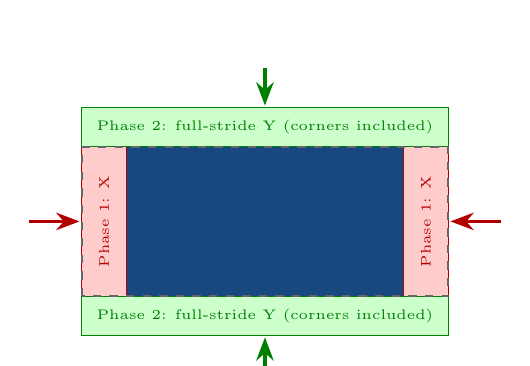
\begin{tikzpicture}[scale=0.95, >=Stealth]
\draw[fill=gray!12, draw=gray!50] (-1.45,-0.52) rectangle (3.45,2.52);
\draw[fill=blue!10, thick, accent] (-0.85,0) rectangle (2.85,2);
\draw[fill=red!20, draw=red!70!black] (-1.45,0) rectangle (-0.85,2);
\draw[fill=red!20, draw=red!70!black] (2.85,0) rectangle (3.45,2);
\draw[fill=green!20, draw=green!50!black] (-1.45,-0.52) rectangle (3.45,0);
\draw[fill=green!20, draw=green!50!black] (-1.45,2) rectangle (3.45,2.52);
\draw[thick, dashed, black!60] (-1.45,0) rectangle (3.45,2);
\node[font=\small\bfseries, accent] at (1,1) {Interior ($n_x^{\text{loc}}\times n_y^{\text{loc}}$)};
\node[font=\tiny, red!70!black, rotate=90] at (-1.15,1) {Phase 1: X};
\node[font=\tiny, red!70!black, rotate=90] at (3.15,1) {Phase 1: X};
\node[font=\tiny, green!50!black] at (1,2.26) {Phase 2: full-stride Y (corners included)};
\node[font=\tiny, green!50!black] at (1,-0.26) {Phase 2: full-stride Y (corners included)};
\draw[->, very thick, red!70!black] (-2.15,1) -- (-1.48,1);
\draw[->, very thick, red!70!black] (4.15,1) -- (3.48,1);
\draw[->, very thick, green!50!black] (1,3.05) -- (1,2.55);
\draw[->, very thick, green!50!black] (1,-1.05) -- (1,-0.55);
\end{tikzpicture}
\caption{Sequential X-then-Y halo exchange (\code{CartDecomp2D}). Phase~1 fills left/right ghosts; Phase~2 transfers full-stride bottom/top bands including corner ghosts.}
\label{fig:mpi_halo}
\end{figure}

\subsection{Unstructured Owner-Computes Decomposition (\code{UnstructuredDecomp})}

\begin{itemize}
\item \textbf{Partitioning:} Sorts cell centroids lexicographically by $(x_c, y_c, c)$ into contiguous balanced rank strips (\code{owner[c]}), defining each rank's \code{active\_cells\_} and incident \code{active\_faces\_}. All QR setup and polynomial solves run only on \code{active\_cells\_}.
\item \textbf{One-Time Halo Schedules (\code{UnstructuredCommSchedule}):} Ranks collect unique remote cells referenced in their 2-ring reconstruction stencils (\code{needed\_u}) and 1-ring adjacent faces (\code{needed\_poly}), transposing request lists once in the solver constructor via \code{MPI\_Alltoall} + \code{MPI\_Alltoallv}.
\item \textbf{Stage Exchanges:} Each RHS evaluation performs two sparse nonblocking point-to-point exchanges: (1) 1-Real \code{u\_sched\_} exchange before reconstruction, and (2) 8-Real \code{CellPoly2} \code{poly\_sched\_} exchange for high-order schemes before active-face flux integration, followed by \code{allreduce\_sum} on boundary fluxes and rank-0 \code{MPI\_Allgatherv} for snapshots/diagnostics.
\end{itemize}

%======================================================================
\section{Benchmark Problems, Verification, and Results}
%======================================================================

Each application runs one canonical benchmark across four solver configurations (\code{--scheme first|\allowbreak tvd|\allowbreak eno|\allowbreak weno|\allowbreak all}); smooth formal EOC checks, grid-aligned controls, \code{Venkatakrishnan}, \code{WENO-JS}, \code{ENO2}, and 4-rank MPI equivalence tests reside in \code{tests/test\_solvers.cpp}.

\subsection{Problem 1: Oblique Diagonal Band on $(0,1)^2$}

\begin{itemize}
\item \textbf{Problem:} $u_t + u_x + u_y = 0$ ($\mathbf{a}=(1,1)$) on $(0,1)^2$, $T=1.0$, $\mathrm{CFL}=0.45$, grids $N\in\{40,80,160,320\}$.
\item \textbf{IC \& BCs:} $u_0(x,y) = \mathbf{1}_{\{|y-x|<0.2\}}$ computed via exact area clipping (\code{intersection\_\allowbreak area\_\allowbreak diagonal\_\allowbreak band}), exact \code{DirichletFaceAvg} inflow at $x=0$ and $y=0$, \code{ZeroGradient} outflow at $x=1, y=1$.
\item \textbf{Metrics:} $E_1, E_2, E_\infty$, midpoint value along $x+y=1$, and $10\text{--}90\%$ front thickness $d_{10\text{--}90}$ along anti-diagonal slices $x+y=0.5$ and $x+y=1.0$.
\end{itemize}

Across a linear contact discontinuity, a scheme of smooth order $p$ converges asymptotically in $L^1$ as $O(h^{p/(p+1)})$ ($0.50$ for $p=1$, $0.67$ for $p=2,3$, $0.83$ for $p=5$). Table~\ref{tab:p1} reports the 4-rank MPI benchmark table ($\max R_M^n \le 1.91\times 10^{-14}$).

\begin{table}[h]
\centering\scriptsize\setlength{\tabcolsep}{4pt}
\caption{Problem 1 (Diagonal Band, 4 ranks): discrete errors, EOCs, front width, bounds, and runtime.}
\label{tab:p1}
\begin{tabular}{@{}lrrrrrrcr@{}}
\toprule
\textbf{Scheme} & \textbf{Grid} & $L^1$ & \code{EOC\_1} & $L^2$ & \code{EOC\_2} & $d_{10\text{--}90}(x+y=1)$ & $[u_{\min}, u_{\max}]$ & \textbf{Time (s)} \\
\midrule
\code{1st-Order} & $40^2$  & $1.477\times 10^{-1}$ & ---  & $2.122\times 10^{-1}$ & ---  & merged ($<0.9$) & $[2.33\times 10^{-10}, 1]$ & 0.003 \\
\code{1st-Order} & $160^2$ & $8.027\times 10^{-2}$ & 0.46 & $1.503\times 10^{-1}$ & 0.24 & 0.12847 & $[2.94\times 10^{-39}, 1]$ & 0.044 \\
\code{1st-Order} & $320^2$ & $5.776\times 10^{-2}$ & 0.47 & $1.281\times 10^{-1}$ & 0.23 & 0.09073 & $[8.64\times 10^{-78}, 1]$ & 1.259 \\
\midrule
\code{TVD-mc}    & $40^2$  & $3.336\times 10^{-2}$ & ---  & $8.680\times 10^{-2}$ & ---  & 0.08684 & $[0, 1]$ & 0.004 \\
\code{TVD-mc}    & $160^2$ & $1.340\times 10^{-2}$ & 0.66 & $5.818\times 10^{-2}$ & 0.30 & 0.02775 & $[0, 1]$ & 0.156 \\
\code{TVD-mc}    & $320^2$ & $8.377\times 10^{-3}$ & 0.68 & $4.690\times 10^{-2}$ & 0.31 & 0.01701 & $[0, 1]$ & 1.811 \\
\midrule
\code{ENO3}      & $40^2$  & $4.073\times 10^{-2}$ & ---  & $8.971\times 10^{-2}$ & ---  & 0.09516 & $[1.03\times 10^{-21}, 1]$ & 0.007 \\
\code{ENO3}      & $160^2$ & $1.678\times 10^{-2}$ & 0.65 & $6.079\times 10^{-2}$ & 0.29 & 0.03381 & $[1.45\times 10^{-85}, 1]$ & 0.390 \\
\code{ENO3}      & $320^2$ & $1.057\times 10^{-2}$ & 0.67 & $4.914\times 10^{-2}$ & 0.31 & 0.01997 & $[1.06\times 10^{-170}, 1]$ & 4.848 \\
\midrule
\code{WENO5-z}   & $40^2$  & $2.587\times 10^{-2}$ & ---  & $6.524\times 10^{-2}$ & ---  & 0.07989 & $[-8.09\times 10^{-5}, 1.00065]$ & 0.028 \\
\code{WENO5-z}   & $160^2$ & $9.138\times 10^{-3}$ & 0.76 & $4.162\times 10^{-2}$ & 0.34 & 0.02255 & $[-5.65\times 10^{-6}, 1.00001]$ & 0.897 \\
\code{WENO5-z}   & $320^2$ & $\mathbf{5.339\times 10^{-3}}$ & \textbf{0.78} & $\mathbf{3.269\times 10^{-2}}$ & \textbf{0.35} & \textbf{0.01187} & $[-1.48\times 10^{-6}, 1]$ & 8.781 \\
\bottomrule
\end{tabular}
\end{table}

\subsection{Problem 2: Unstructured Tube Transport on $(0,4)\times(0,1)$}

\begin{itemize}
\item \textbf{Problem:} $u_t + u_x = 0$ ($\mathbf{a}=(1,0)$) on $(0,4)\times(0,1)$, $T=2.0$, $\mathrm{CFL}=0.45$, zero inflow at $x=0$.
\item \textbf{IC \& Geometry:} Exact cell-averaged square patch $S_0 = [0.5,1.0]\times[0.25,0.75]$ advected to $S(T)=[2.5,3.0]\times[0.25,0.75]$ (exact mass $0.25$, $\sigma_x=\sigma_y=0.5/\sqrt{12}=0.144338$).
\item \textbf{Two Mesh Hierarchies ($\code{ref}=0,1,2,3 \implies 264, 1056, 4224, 16896$ triangles):}
  \begin{itemize}
    \item \code{--mesh nested}: $22\times 6$ Lloyd-smoothed Delaunay base mesh (\code{jitter=0.35, smooth=5}, constant $q_{\min}=0.815438$, $h_{\text{diam}}=0.2466\to 0.03083$) uniformly refined 1-to-4.
    \item \code{--mesh irregular}: independent unsmoothed Delaunay meshes (\code{jitter=0.45, smooth=0}, $q_{\min}=0.6994\to 0.5656$, $h_{\text{diam}}=0.2802\to 0.03846$).
  \end{itemize}
\item \textbf{Diagnostics:} cross-stream leakage \code{cross\_leak} (mass outside $y\in[0.25,0.75]$), streamwise spill \code{stream\_spill} (mass in $y\in[0.25,0.75]\setminus[2.5,3.0]$), and moments $(\sigma_x,\sigma_y)$.
\end{itemize}

\begin{table}[h]
\centering\scriptsize\setlength{\tabcolsep}{2.9pt}
\caption{Problem 2 (Unstructured Tube Transport, finest \code{ref=3}, $16{,}896$ cells, 4 ranks): nested vs.\ irregular.}
\label{tab:p2}
\begin{tabular}{@{}llrrrrccr@{}}
\toprule
\textbf{Mesh} & \textbf{Scheme} & $L^1$ & \code{EOC\_1} & \textbf{Cross leak} & \textbf{Stream spill} & $(\sigma_x,\sigma_y)$ & $[u_{\min}, u_{\max}]$ & \textbf{Time (s)} \\
\midrule
\code{nested}    & \code{1st-Tri}  & $1.028\times 10^{-1}$ & 0.44 & $4.900\times 10^{-3}$ & $4.959\times 10^{-2}$ & $(0.1921,0.1450)$ & $[0, 0.9518]$ & 0.286 \\
\code{nested}    & \code{TVD-Tri}  & $3.421\times 10^{-2}$ & 0.69 & $3.709\times 10^{-3}$ & $1.651\times 10^{-2}$ & $(0.1507,0.1446)$ & $[-5.92\times 10^{-14}, 1]$ & 0.885 \\
\code{nested}    & \code{ENO3-Tri} & $3.113\times 10^{-2}$ & 0.69 & $3.655\times 10^{-3}$ & $1.503\times 10^{-2}$ & $(0.1495,0.1447)$ & $[-0.00285, 1.00885]$ & 6.227 \\
\code{nested}    & \code{WENO-Tri} & $\mathbf{3.020\times 10^{-2}}$ & 0.67 & $3.695\times 10^{-3}$ & $\mathbf{1.456\times 10^{-2}}$ & $(0.1490,0.1447)$ & $[-0.00378, 1.00397]$ & 5.128 \\
\midrule
\code{irregular} & \code{1st-Tri}  & $1.490\times 10^{-1}$ & 0.45 & $2.841\times 10^{-2}$ & $4.914\times 10^{-2}$ & $(0.2004,0.1610)$ & $[0, 0.9274]$ & 0.335 \\
\code{irregular} & \code{TVD-Tri}  & $4.632\times 10^{-2}$ & 0.72 & $1.054\times 10^{-2}$ & $1.592\times 10^{-2}$ & $(0.1499,0.1465)$ & $[-4.37\times 10^{-14}, 1]$ & 1.238 \\
\code{irregular} & \code{ENO3-Tri} & $4.204\times 10^{-2}$ & 0.75 & $9.881\times 10^{-3}$ & $1.433\times 10^{-2}$ & $(0.1487,0.1464)$ & $[-3.34\times 10^{-7}, 1.00009]$ & 9.712 \\
\code{irregular} & \code{WENO-Tri} & $\mathbf{4.148\times 10^{-2}}$ & \textbf{0.76} & $9.810\times 10^{-3}$ & $\mathbf{1.409\times 10^{-2}}$ & $(0.1486,0.1463)$ & $[-0.00042, 1.00056]$ & 8.474 \\
\bottomrule
\end{tabular}
\end{table}

Removing Lloyd smoothing and nested refinement increases cross-stream leakage by $5.8\times$ for \code{1st-Tri} and $2.65\times$ for \code{WENO-Tri}, and raises overall $L^1$ error by $\sim 37\%$ while preserving full stencil stability and $\max R_M^n \le 2.165\times 10^{-15}$.

\subsection{Problem 3: KPP Nonconvex Rotating Wave on $(-2.5,2.5)^2$}

\begin{itemize}
\item \textbf{Problem:} $u_t + (\sin u)_x + (\cos u)_y = 0$ on $(-2.5,2.5)^2$, $T=1.0$, $\mathrm{CFL}=0.45$, global Rusanov $\alpha=1$, $N\in\{100,200,400,800\}$.
\item \textbf{IC \& BCs:} Exact disk--cell fractions (\code{disk\_intersection\_area\_rect}) with $u_0 = \frac{7\pi}{2}\approx 10.995574$ inside $x^2+y^2 \le 1$ and $u_0 = \frac{\pi}{4}\approx 0.785398$ outside; fixed \code{DirichletExact} $u = \pi/4$ on all four boundaries.
\item \textbf{Reference:} No closed-form elementary analytical solution exists in 2D at $T=1$. Quantitative comparison uses cell-averaged restriction of a $1600\times 1600$ 1st-order monotone Rusanov reference ($1423$ steps, $15.53\,\text{s}$ on 4 ranks, $u\in[0.785398,10.9956]$, $\max R_M^n = 1.58\times 10^{-12}$).
\end{itemize}

\begin{table}[h]
\centering\scriptsize\setlength{\tabcolsep}{3.2pt}
\caption{Problem 3 (KPP, 4 ranks): discrepancy against the $1600\times 1600$ monotone Rusanov reference.}
\label{tab:p3}
\begin{tabular}{@{}lrrrrrrrcr@{}}
\toprule
\textbf{Scheme} & $L^1(100^2)$ & $L^1(200^2)$ & $L^1(400^2)$ & $L^1(800^2)$ & $L^2(800^2)$ & $L^\infty(800^2)$ & \textbf{Bounds at} $800^2$ & $\max R_M^n$ & \textbf{Time (s)} \\
\midrule
\code{1st-Order}  & 4.052 & 2.250 & 1.128 & 0.431 & 0.726 & 4.321 & $[0.785398, 10.9956]$ & $7.18\times 10^{-13}$ & 4.189 \\
\code{TVD-minmod} & 1.431 & 0.667 & \textbf{0.246} & \textbf{0.280} & \textbf{0.602} & 4.395 & $[0.785398, 10.9956]$ & $8.24\times 10^{-13}$ & 7.054 \\
\code{ENO3}       & 1.756 & 0.977 & 0.554 & 0.534 & 1.096 & 5.380 & $[0.785398, 10.9956]$ & $5.33\times 10^{-13}$ & 17.522 \\
\code{WENO5-z}    & 2.215 & 1.611 & 1.305 & 1.263 & 2.104 & 5.930 & $[0.785394, 10.9956]$ & $6.89\times 10^{-13}$ & 40.563 \\
\bottomrule
\end{tabular}
\end{table}

\paragraph{The Nonconvex KPP Entropy Paradox.}
Because $\sin u$ and $\cos u$ reverse convexity inside $[\pi/4, 7\pi/2]$, the true entropy solution is a twisted 2D composite wave (shock + rarefaction). Dimension-by-dimension high-order reconstructions carry far less numerical viscosity near sonic/inflection points than 1st-order Rusanov, causing spurious composite-wave corner twisting to persist under refinement: at $800^2$, \code{WENO5-z} exhibits nearly $3\times$ the $L^1$ discrepancy of \code{1st-Order} and $>4.5\times$ that of \code{TVD-minmod} (which itself turns upward between $400^2$ and $800^2$), reproducing the Kurganov--Petrova--Popov (2007) benchmark finding.

\subsection{Automated Verification Suite (\code{tests/})}

Both serial and 4-rank MPI builds pass all 6 core tests (\code{test\_core}) and all 13 solver verification tests (\code{test\_solvers}):
\begin{itemize}
\item \textbf{Core Infrastructure:} 1D/2D quadrature accuracy, dense LU/QR orthogonality, sparse SGS-CG (30 iters) \& SGS-BiCGSTAB (8 iters) on 2D Poisson, unstructured mesh generation ($q_{\min}$ \& conservation), RK convergence orders ($\mathrm{RK2}=2.013$, $\mathrm{RK3}=3.015$, $\mathrm{RK4}=4.021$), VTK/CSV output.
\item \textbf{Structured Formal EOCs:} Smooth periodic diagonal sine wave recovers 2nd/3rd-order TVD superconvergence ($\mathrm{EOC}_1 = 2.987$ for \code{MC}), 3rd-order \code{ENO3} ($\mathrm{EOC}_1 = 2.988$, $L^\infty$ $\mathrm{EOC}=3.010$; smooth nonlinear 2D KPP $\mathrm{EOC}=2.989$), and 5th-order \code{WENO5-Z} ($\mathrm{EOC}_1 = 4.965$, $L^\infty$ $\mathrm{EOC}=4.966$; smooth nonlinear 2D KPP with RK4 $\mathrm{EOC}=4.935$).
\item \textbf{Unstructured Smooth EOCs:} Smooth $\cos^6$ bump and $C^\infty$ $\sin(\pi x)\sin(\pi y)$ verify Venkatakrishnan TVD ($\mathrm{EOC}_1=1.873$), \code{ENO3} ($\mathrm{EOC}_1=2.276$), and $P^2$ \code{WENO-Z} ($\cos^6$ $\mathrm{EOC}_1=2.349$; $\sin$ $\mathrm{EOC}_1=3.088$, $L^\infty$ $\mathrm{EOC}=2.739$).
\item \textbf{MPI Pointwise Equivalence:} 4-rank runs agree with serial results to $<10^{-14}$ across periodic structured WENO5-Z, non-periodic inflow/extrapolation WENO5-Z, unstructured Venkatakrishnan TVD, and unstructured $P^2$ WENO-Z.
\end{itemize}

\end{document}
